\documentclass[11pt]{article}
\usepackage[spanish]{babel}
\usepackage{natbib}
\usepackage{url}
\usepackage[utf8x]{inputenc}
\usepackage{amsmath}
\usepackage{amssymb}
\usepackage{graphicx}
\graphicspath{{images/}}
\usepackage{parskip}
\usepackage{fancyhdr}
\usepackage{vmargin}
\usepackage{natbib}
\usepackage{apalike}
\usepackage{longtable}

\setmarginsrb{3 cm}{2.5 cm}{3 cm}{2.5 cm}{1 cm}{1.5 cm}{1 cm}{1.5 cm}

\title{Programas}						% Title
\author{J. Eduardo Sánchez Posadas}					%Author
\date{\today}											% Date

\makeatletter
\let\thetitle\@title
\let\theauthor\@author
\let\thedate\@date
\makeatother

\pagestyle{fancy}
\fancyhf{}
\rhead{Estructuras de Datos}
\lhead{\thetitle}
\rfoot{\thepage}
\lfoot{FES Aragón - UNAM}

\begin{document}

%%%%%%%%%%%%%%%%%%%%%%%%%%%%%%%%%%%%%%%%%%%%%%%%%%%%%%%%%%%%%%%%%%%%%%%%%%%%%%%%%%%%%%%%%

\begin{titlepage}
	\centering
    \vspace*{0.5 cm}
    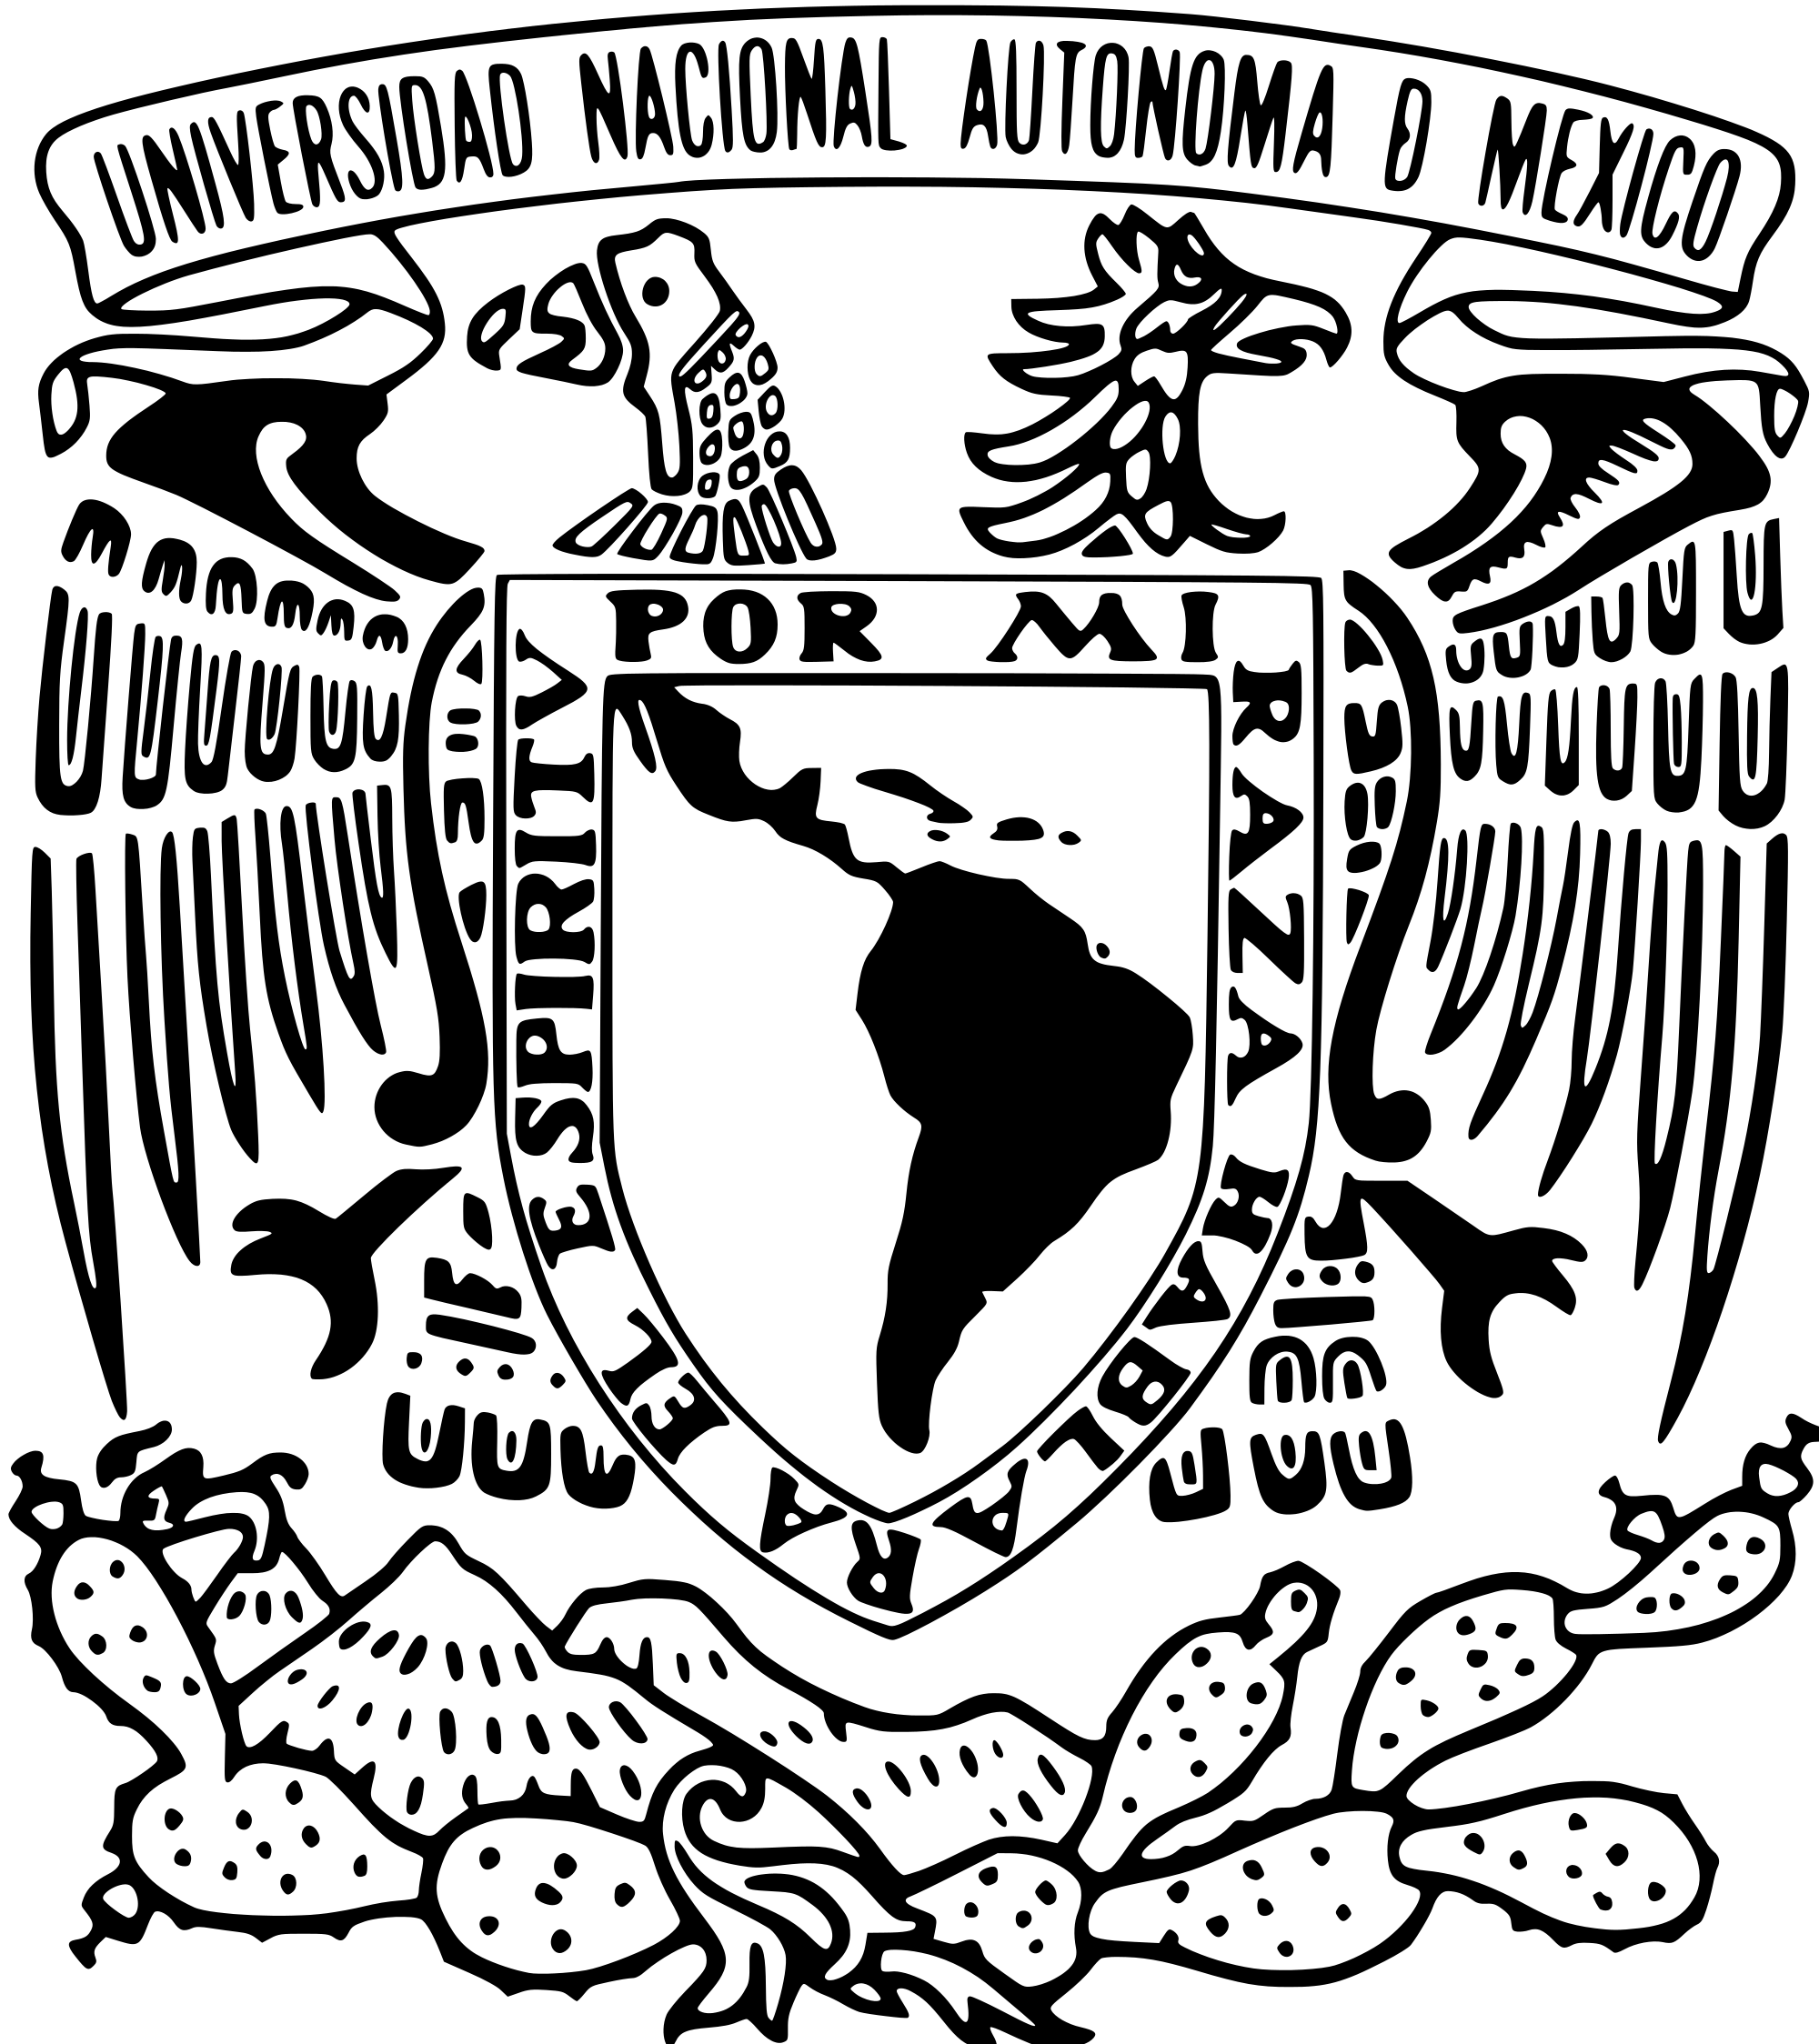
\includegraphics[scale=0.05]{pics/escudo.png} \\[1.0 cm]	% University Logo
    \textsc{\Large Universidad Nacional Autónoma de México}\\[2.0 cm]	% University Name
	\textsc{\Large FES Aragón\\ Ingeniería en Computación}\\[0.5 cm]								% Course Code
	\textsc{\Large Estructuras de Datos \\ con Java}\\[0.5 cm]	% Course Name
	\rule{\linewidth}{0.2 mm} \\[0.4 cm]
	{ \huge \bfseries \thetitle}\\
	\rule{\linewidth}{0.2 mm} \\[1.5 cm]
	 			{Autor: \large \theauthor}
% 	\begin{minipage}{0.4\textwidth}
% 		\begin{flushleft} \large
% 			\emph{Nombre: Nombre(s) Apellido(s]}\\
%
% 			\end{flushleft}
% 			\end{minipage}~
% 			\begin{minipage}{0.4\textwidth}
% 			\begin{flushright} \large
% 			\emph{Número de Cuenta} \\
% 											% Your Student Number
% 		\end{flushright}
% 	\end{minipage}\\[2 cm]
	
	{\large \thedate}\\[2 cm]
 
	\vfill
	
\end{titlepage}
% Please add the folloswing required packages to your document preamble:
% \usepackage{longtable}
% Note: It may be necessary to compile the document several times to get a multi-page table to line up properly
\begin{longtable}[c]{|c|c|c|c|}
\hline
\textbf{ID}              & \textbf{Tema}                                & \textbf{Actividad}                                                      & \textbf{Descripción}                                                                                                                                   \\ \hline
\endfirsthead
%
\endhead
%
$1_i$                     & Estructuras básicas                          & Reseña artículo                                                         & \begin{tabular}[c]{@{}c@{}}Realizar una reseña de una \\ cuartilla sobre el artículo\end{tabular}                                                      \\ \hline
2                        & Estructuras básicas                          & Estándar IEEE754                                                        & \begin{tabular}[c]{@{}c@{}}Realizar una clase que convierta\\ números al estándar IEEE754\end{tabular}                                                 \\ \hline
3                        & Estructuras lineales                         & \begin{tabular}[c]{@{}c@{}}Implementación\\ de ListaSimple\end{tabular} & \begin{tabular}[c]{@{}c@{}}Clase donde se implementan \\ todos los métodos de una lista\\ Ligada simple\end{tabular}                                   \\ \hline
4                        & Estructuras lineales                         & Pruebas de ListaSimple                                                  & \begin{tabular}[c]{@{}c@{}}Tres pruebas de la lista simple: \\ Integers, String, clase Automóvil\end{tabular}                                          \\ \hline
5                        & Estructuras lineales                         & Paréntesis                                                              & \begin{tabular}[c]{@{}c@{}}Verificar que los paréntesis en una \\ expresión estén balanceados\end{tabular}                                             \\ \hline
6                        & Estructuras lineales                         & Signos de agrupamiento                                                  & \begin{tabular}[c]{@{}c@{}}Verificar que los paréntesis en una \\ expresión estén balanceados y \\ colocados de manera correcta\end{tabular}           \\ \hline
7!                       & Estructuras lineales                         & Verificar operaciones                                                   & \begin{tabular}[c]{@{}c@{}}Verificar que una operación\\ esté bien escrita\end{tabular}                                                                \\ \hline
8                        & Estructuras lineales                         & Conversión infijo-posfijo                                               & \begin{tabular}[c]{@{}c@{}}Convertir una expresión infija\\ a una prefija, y viceversa\end{tabular}                                                    \\ \hline
9                        & Estructuras lineales                         & Torres de Hanoi                                                         & \begin{tabular}[c]{@{}c@{}}Simular con pilas el juego de\\ las torres de Hanoi\end{tabular}                                                            \\ \hline
10                       & Estructuras lineales                         & Supermercado                                                            & \begin{tabular}[c]{@{}c@{}}Simular con una cola la fila\\ de un supermercado\end{tabular}                                                              \\ \hline
$11_{i}$                    & Estructuras no lineales                      & Preguntas                                                               & Responder a las pregunas                                                                                                                               \\ \hline
\multicolumn{1}{|l|}{12} & \multicolumn{1}{l|}{Estructuras no lineales} & Grafo Metro                                                             & \begin{tabular}[c]{@{}c@{}}Implementar en una matriz de un\\  grafo no dirigido de la red del metro\\ e imprimirlo en un archivo de texto\end{tabular} \\ \hline
\multicolumn{1}{|l|}{13} & \multicolumn{1}{l|}{Estructuras no lineales} & Arboles de expresion                                                    & \begin{tabular}[c]{@{}c@{}}Dar los arboles de expresión para las\\ operaciones dadas\end{tabular}                                                      \\ \hline
\end{longtable}
\newpage
\section{Apéndice A. Diagrama de clases para la actividad 10}

\newpage

\section{Apéndice A}

\newpage

\section{Apéndice A}

\newpage

\section{Apéndice A}

\newpage
\end{document}
